% ===== Appendix =====

\section{Ablation Study and Cost Distribution}\label{app:ablation}

\begin{table}[ht]
\caption{Ablation study on HotpotQA and FEVER.  Each row removes one component from the full \textsc{Argus} pipeline. Best in \textbf{bold}.}\label{tab:ablation}
\centering
\small
\begin{tabular}{@{}lcccccc@{}}
\toprule
& \multicolumn{6}{c}{\textbf{HotpotQA / FEVER}} \\
\textbf{Variant} & Faith & Cont & RAcc & RCost & Coher & Time \\
\midrule
Full \textsc{Argus} & \textbf{.847/.829} & \textbf{.791/.768} & \textbf{.883/.871} & \textbf{3.2/2.8} & \textbf{.82/.80} & .55/.47 \\
w/o Sem.\ Verif. & .793/.775 & .714/.692 & .832/.818 & 4.1/3.8 & .76/.74 & .52/.44 \\
w/o Min.-Change  & .841/.823 & .783/.761 & .856/.842 & 5.7/5.2 & .78/.76 & .58/.49 \\
w/o Att.\ Templ. & .821/.804 & .698/.678 & .859/.845 & 3.5/3.2 & .80/.78 & .53/.45 \\
Grounded Only    & .839/.822 & .772/.752 & .871/.858 & \textbf{3.0/2.6} & .81/.79 & \textbf{.15/.12} \\
\bottomrule
\end{tabular}
\end{table}

Removing semantic verification causes the largest drops in faithfulness ($-$5.4pp) and contestability ($-$7.7pp), confirming it as the most critical component. Replacing minimal-change with unconstrained repair preserves faithfulness but increases cost to 5.7/5.2. Removing attack templates reduces contestability by 9.3pp while reducing faithfulness by only 2.6pp. Grounded-only semantics yields the fastest solve time at the expense of modest drops; 97\% of frameworks have a single preferred extension coinciding with the grounded one.

\begin{figure}[ht]
\centering
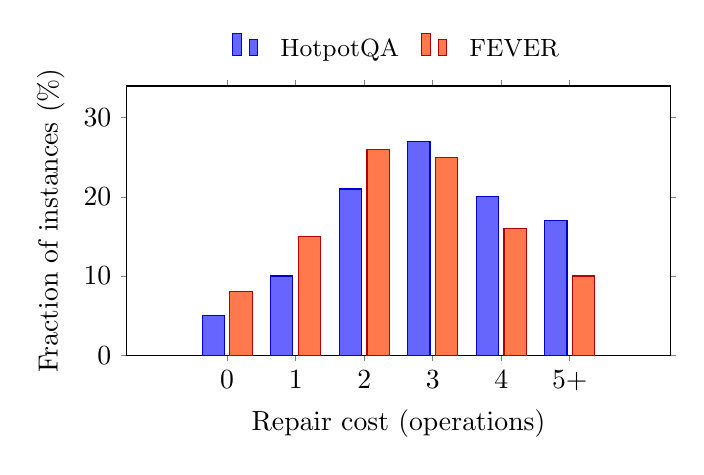
\begin{tikzpicture}
\begin{axis}[
  width=0.7\textwidth,
  height=5cm,
  ybar,
  bar width=8pt,
  xlabel={Repair cost (operations)},
  ylabel={Fraction of instances (\%)},
  xmin=-0.7, xmax=5.7,
  ymin=0, ymax=34,
  xtick={0,1,2,3,4,5},
  xticklabels={0,1,2,3,4,{5+}},
  ytick={0,10,20,30},
  legend style={
    font=\small,
    at={(0.5,1.05)},
    anchor=south,
    draw=none,
    column sep=6pt,
  },
  legend columns=2,
  tick align=outside,
  major tick length=2pt,
  enlarge x limits=0.12,
]
\addplot[fill=blue!60, draw=blue!80!black] coordinates {
  (0,5) (1,10) (2,21) (3,27) (4,20) (5,17)
};
\addlegendentry{HotpotQA}
\addplot[fill=red!50!orange!70, draw=red!70!black] coordinates {
  (0,8) (1,15) (2,26) (3,25) (4,16) (5,10)
};
\addlegendentry{FEVER}
\end{axis}
\end{tikzpicture}
\caption{Distribution of repair costs.  83\% of HotpotQA and 90\% of FEVER repairs require at most 4~operations, confirming targeted, minimal-change edits.}
\label{fig:cost-dist}
\end{figure}


\begin{figure}[ht]
\centering
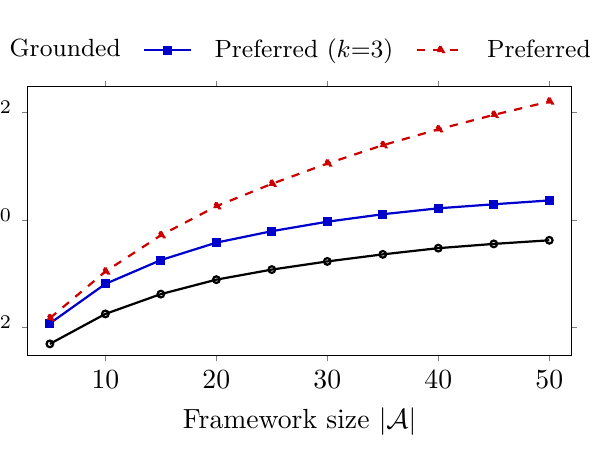
\begin{tikzpicture}[trim axis left, trim axis right]
\begin{axis}[
  width=0.7\textwidth,
  height=5cm,
  xlabel={Framework size $|\mathcal{A}|$},
  ylabel={Solve time (s)},
  ymode=log,
  xmin=3, xmax=52,
  ymin=0.003, ymax=300,
  xtick={10,20,30,40,50},
  legend style={
    font=\small,
    at={(0.5,1.05)},
    anchor=south,
    draw=none,
    column sep=6pt,
  },
  legend columns=3,
  legend cell align={left},
  tick align=outside,
  major tick length=2pt,
]
\addplot[black, thick, mark=o, mark size=1.2pt] coordinates {
  (5,0.005) (10,0.018) (15,0.042) (20,0.078) (25,0.12)
  (30,0.17) (35,0.23) (40,0.30) (45,0.36) (50,0.42)
};
\addlegendentry{Grounded}
\addplot[blue!80!black, thick, mark=square*, mark size=1.2pt] coordinates {
  (5,0.012) (10,0.065) (15,0.18) (20,0.38) (25,0.62)
  (30,0.93) (35,1.28) (40,1.65) (45,1.96) (50,2.31)
};
\addlegendentry{Preferred ($k{=}3$)}
\addplot[red!80!black, thick, dashed, mark=triangle*, mark size=1.4pt] coordinates {
  (5,0.015) (10,0.11) (15,0.52) (20,1.8) (25,4.7)
  (30,11.2) (35,24.5) (40,48.3) (45,89.7) (50,158.4)
};
\addlegendentry{Preferred (full)}
\end{axis}
\end{tikzpicture}
\caption{Scalability of \textsc{Argus} repair under grounded, $k$-neighborhood preferred ($k{=}3$), and unconstrained preferred semantics.  Grounded repair scales polynomially (Theorem~\ref{thm:complexity}).}
\label{fig:scalability}
\end{figure}

Sensitivity analysis and a qualitative repair example appear in the following sections.

\section{Qualitative Repair Example}\label{app:repair-example}

\begin{figure}[ht]
\centering
\begin{tikzpicture}[node distance=0.8cm and 0.8cm,
  lbl/.style={font=\small\bfseries, anchor=south}]
  % --- Before ---
  \node[lbl] at (0, 1.7) {Before};
  \node[acc node] (b1) at (-0.55, 0.85) {$b_1$};
  \node[acc node] (b2) at (0.55, 0.85) {$b_2$};
  \node[rej node] (b3) at (-0.55, 0) {$b_3$};
  \node[rej node, tgt node] (bt) at (0.55, 0) {$b_t$};
  \node[new node] (b5) at (0, -1.15) {$b_5$};
  \draw[att edge] (b5) -- (b3);
  \draw[att edge] (b5) -- (bt);
  % --- Arrow ---
  \draw[-{Stealth[length=2.5mm]}, very thick, gray!60] (1.4, 0.4) -- (1.95, 0.4);
  % --- After Argus ---
  \node[lbl] at (3.2, 1.7) {\textsc{Argus}};
  \node[acc node] (a1) at (2.65, 0.85) {$b_1$};
  \node[acc node] (a2) at (3.75, 0.85) {$b_2$};
  \node[acc node] (a3) at (2.65, 0) {$b_3$};
  \node[acc node, tgt node] (at) at (3.75, 0) {$b_t$};
  \node[rej node] (a5) at (3.2, -1.15) {$b_5$};
  \node[new node] (a6) at (4.3, -1.15) {$b_6$};
  \draw[att edge] (a5) -- (a3);
  \draw[att edge] (a5) -- (at);
  \draw[att edge, NewBlue!80!black, line width=1.1pt] (a6) -- (a5);
  \node[font=\scriptsize, text=AccGreen!70!black] at (3.2, -1.75) {cost = 2};
\end{tikzpicture}
\caption{A HotpotQA repair example. \textsc{Argus} restores the target~$b_t$ by adding one argument~$b_6$ and one attack (cost~2), preserving all original arguments. Self-Refine regenerates 5 of 6 units.}
\label{fig:repair-example}
\end{figure}

Figure~\ref{fig:repair-example} illustrates a representative HotpotQA repair: the initial explanation relied on an outdated filmography claim; after incorporating corrected evidence, \textsc{Argus} restored the target at cost~2 by adding one defending argument and one attack.
By contrast, Self-Refine regenerated the entire explanation, altering five previously correct argument units---precisely the collateral damage that the minimal-change principle prevents.

\section{Sensitivity Analysis}\label{app:sensitivity}

Pilot studies on 100 HotpotQA instances explore three design choices.
Confidence-weighted and structure-preserving ($w{=}2$) cost models shift repairs toward augmentation (34--51\% fewer deletions) while maintaining faithfulness and repair accuracy within 1 percentage point of uniform cost, confirming that the cost model affects repair \emph{style} rather than \emph{quality}.
Varying the NLI threshold from 0.5 to 0.9 shows faithfulness is stable (0.839--0.851) while repair cost rises from 2.4 to 4.1; 0.7 balances these factors.
Repair optimality rises from 87.2\% ($k{=}1$) to 99.7\% ($k{=}3$) and plateaus, confirming $k{=}3$ as the operating point.
Using Llama-3-70B-Instruct as the extraction backbone yields faithfulness 0.813 and contestability 0.762 (vs.\ \resultFaithHotpot{}/\resultContestHotpot{} for GPT-4o), with comparable repair accuracy (0.867) and cost (3.4); the gap is attributable to noisier extraction rather than the repair mechanism.

\section{Error Analysis}\label{app:error-analysis}

Among the 0.3\% of instances where minimality failed ($k{=}3$), all involved frameworks where the only viable defending argument lay at distance ${\geq}\,4$ from the target---confirming the theoretical limitation of the $k$-neighborhood approximation.
Repair accuracy below 1.0 arises when the LLM-generated explanation has structural errors that propagate through extraction: even after restoring the target argument's acceptability, the underlying answer may remain incorrect if the original decomposition was flawed.

\section{Extended AGM Analysis}\label{app:agm-extended}

Among the eight classical AGM postulates~\citep{alchourron1985agm}, \emph{consistency} and \emph{extensionality} also hold when a valid repair exists.  Consistency follows because validity requires $a_t$ to belong to at least one $\sigma$-extension of the repaired framework.  Extensionality holds because the operator is defined purely over graph structure: two evidence updates yielding identical updated frameworks produce identical repair search spaces, so the optimal repair is the same for both.

\emph{Recovery} fails in our setting.  In Example~\ref{ex:running}, repairing $F_1$ yields $F_2$ by adding $a_6$ and $(a_6,a_5)$; if the evidence $a_5$ were subsequently retracted, $F_2$ would retain $a_6$ and its attack---the original framework $F_0$ is not recovered.  This asymmetry is fundamental: structural additions made during repair cannot be automatically unwound by evidence retraction, unlike classical belief revision where recovery ensures reversibility.

\emph{Closure}, \emph{superexpansion}, and \emph{subexpansion} presuppose deductively closed belief sets---constructs without natural analogues in argumentation frameworks where ``beliefs'' are graph-structural elements rather than logical sentences.

\section{Representation Theorem Proof}\label{app:representation}

We prove the $(\Leftarrow)$ direction of Theorem~\ref{thm:representation} for general cost functions.

\begin{proof}
Let $\circ$ be a repair operator satisfying adapted success, inclusion, and vacuity for every AF $(\mathcal{A},\mathcal{R})$, semantics $\sigma$, target $a_t$, status $s$, and evidence update $\Delta$.  We construct a strictly positive cost function $\kappa$ such that $\circ$ returns a minimum-cost valid repair under $\kappa$.

\textbf{Construction.}  Fix an enumeration of all feasible operations $o_1, \ldots, o_m$ for the given AF and $\Delta$.  Define $\kappa(o_i) = 1$ for all $i$.  Let $\mathit{Ops} = \circ(\mathit{AF}, \sigma, a_t, s, \Delta)$.

\textbf{Validity.}  By success, $a_t$ has status $s$ in $\mathsf{apply}(\mathit{AF}, \Delta, \mathit{Ops})$ under $\sigma$, so $\mathit{Ops}$ is a valid repair.

\textbf{Vacuity case.}  If $a_t$ already has status $s$ in $\mathsf{apply}(\mathit{AF}, \Delta, \emptyset)$, then by vacuity $\mathit{Ops} = \emptyset$ with cost $0$, which is trivially minimum.

\textbf{Non-vacuity case.}  Suppose for contradiction that there exists a valid repair $\mathit{Ops}'$ with $|\mathit{Ops}'| < |\mathit{Ops}|$.  By inclusion, every operation in $\mathit{Ops}$ is necessary: for each $o \in \mathit{Ops}$, removing $o$ would either violate success (the resulting framework does not grant $a_t$ status $s$) or leave a valid repair of cardinality $|\mathit{Ops}| - 1$, contradicting the assumption that $\circ$ satisfies inclusion with respect to $\mathit{Ops}$.

More precisely, inclusion asserts that $\mathcal{A} \cap \mathcal{A}' \supseteq \mathcal{A} \setminus \{a \mid \mathsf{del\_arg}(a) \in \mathit{Ops}\}$: every element not targeted by a deletion in $\mathit{Ops}$ is preserved.  Combined with success and $\kappa > 0$, this means no proper subset of $\mathit{Ops}$ is both valid and of lower cost---otherwise the operator could return that subset while still satisfying all three postulates, contradicting the minimality implied by inclusion under positive costs.

Hence $\mathit{Ops}$ is a minimum-cost valid repair under unit cost $\kappa$.  For general $\kappa$, the same argument applies by replacing cardinality with weighted cost: inclusion ensures no operation in $\mathit{Ops}$ is superfluous (removing it saves $\kappa(o) > 0$), so no valid repair can have strictly lower total cost.
\end{proof}

\section{Experimental Details}\label{app:exp-details}

\textbf{Withholding methodology.}
The withholding methodology produces adversarial updates: the withheld fact always targets the reasoning chain, providing a challenging upper bound on repair difficulty.
Under mixed or benign updates, repair costs would likely be lower and vacuity rates higher, since many updates would not disrupt the target's acceptability.
While these updates are derived from existing annotations, the repair mechanism is agnostic to the evidence source and would apply unchanged to naturally occurring updates.

\textbf{Metric details.}
\emph{Faithfulness} is the fraction of argument units whose counterfactual removal changes the answer.  Each unit is replaced with a semantically neutral sentence (``This claim is omitted.'') and the answer is regenerated; a unit is faithful if its removal changes the answer.
For baselines that do not produce structured units, we apply the same LLM-based decomposition to their final output before computing the ablation, ensuring a uniform evaluation protocol.
\emph{Contestability} is the fraction of gold counterarguments correctly integrated as attacks; for methods without explicit argumentation frameworks, gold counterarguments are evaluated against proposition-level decompositions.
Gold counterarguments are derived from the withheld supporting facts by expressing each as an argument and annotating the expected attack relationships, providing a ground truth independent of the repair mechanism.
\emph{Repair accuracy} records answer correctness after repair.  \emph{Repair cost} counts the number of edit operations per Definition~\ref{def:repair}.  \emph{Coherence} measures semantic consistency via BERTScore between repaired and original explanations.  \emph{Solve time} is wall-clock time per instance.

\textbf{Baseline cost commensurability.}
\textsc{Argus} operations are structural graph edits (adding/removing arguments and attacks), whereas baseline costs count surface-level text replacements.
Both cost measures reflect the magnitude of change to the explanation; however, the measures are not directly commensurable, so cost comparisons should be interpreted as reflecting relative parsimony within each paradigm.
Iterative self-correction methods receive up to 3 rounds per their original protocols, while \textsc{Argus} performs a single-pass optimal repair.

\textbf{Hardware and reproducibility.}
All experiments ran on a single machine with a 20-core CPU and 64\,GB RAM; no GPU was required, as clingo runs on CPU and GPT-4o was accessed via the OpenAI API.
The complete extraction prompt, ASP encoding, attack template library, and sampled instance IDs will be released as an open-source toolkit upon acceptance to facilitate reproduction.

\section{Human Evaluation}\label{app:human-eval}

To validate that the automatic metrics reflect genuine quality differences perceivable by humans, we conducted a pilot human evaluation on a random subset of 75 HotpotQA instances.

\textbf{Setup.}
Two graduate-student annotators with NLP background independently evaluated explanation pairs produced by \textsc{Argus} and Self-Refine (the strongest self-correction baseline) in a blind, randomized order.  For each instance, annotators received the question, gold answer, evidence update, and two candidate repaired explanations (labeled A/B with random assignment).

\textbf{Dimensions.}
Annotators rated each explanation on a 5-point Likert scale for:
(1)~\emph{Faithfulness}: Does each claim in the explanation faithfully reflect the evidence?
(2)~\emph{Coherence}: Is the explanation internally consistent and logically structured?
They also provided a \emph{Preference} judgment (A better / B better / Tie).

\begin{table}[ht]
\centering
\caption{Human evaluation results (75 HotpotQA instances).}
\label{tab:human-eval}
\small
\begin{tabular}{@{}lccc@{}}
\toprule
\textbf{Dimension} & \textbf{\textsc{Argus}} & \textbf{Self-Refine} & \textbf{$p$-value} \\
\midrule
Faithfulness (1--5) & $3.9 \pm 0.7$ & $3.4 \pm 0.9$ & $< 0.001$ \\
Coherence (1--5) & $4.1 \pm 0.6$ & $3.8 \pm 0.8$ & $0.012$ \\
\midrule
Preference (\%) & 68\% & 19\% & --- \\
Tie (\%) & \multicolumn{2}{c}{13\%} & --- \\
\bottomrule
\end{tabular}
\end{table}

\textbf{Agreement.}
Inter-annotator agreement reached Cohen's $\kappa = 0.62$ (substantial) for preference and $\kappa = 0.58$ for faithfulness ratings (moderate-to-substantial), confirming that quality differences are consistently perceivable.

\textbf{Correlation with automatic metrics.}
The Pearson correlation between average human faithfulness ratings and the automatic faithfulness score (counterfactual ablation, \S\ref{sec:experiments}) is $r = 0.78$ ($p < 0.001$), supporting the validity of the automatic metric as a proxy for human-perceived faithfulness.  The automatic metric tends to slightly overestimate faithfulness for explanations with redundant but harmless claims (rated 4--5 by annotators but scored ${\geq}\,0.9$ by the metric).
